\section{Principal Component Analysis}



\subsection{PCA and preprocessing}

Let $\mbf A$ be some matrix in $\mathbb R^{n \times d}$ and $i$'th column vector
$\mbf a_i$ and column mean $\bar{\mbf a}$. Let then $\mbf C$ be the
column-centering of $\mbf A$ with where each column vector $\mbf c_i$ is given
by $\mbf c_i = \mbf a_i - \bar{\mbf a}$.


Consider the sum of all $d$ column vectors of $\mbf C$:

\begin{align*}
  \sum_{i = 1}^d \mbf c_i &= \sum_{i = 1}^d \left(\mbf a_i - \bar{\mbf a}\right)\\
                          &= \sum_{i = 1}^d (\mbf a_i) \,  - d * \bar{\mbf a}
\end{align*}

Using the definition of $\bar {\mbf a}$:

\begin{align}
  &= \sum_{i = 1}^d (\mbf a_i) - d * \left(\frac{1}{d}\sum_{i = 1}^d \mbf a_i \right)\nonumber\\
  &= \mbf 0_n \label{eq:combination_all}
\end{align}

And so we see that the linear combination of all columns is $\mbf 0_n$, the
zero-vector of length $n$ (note: $n$, not $d$). This implies that any column
$\mbf c_i$ of $\mbf C$ is a linear combination of the other $d - 1$ columns.
Let's see how:
% In
% particular, the $k$'th column is equal to the sum of the other $d - 1$ columns
% times negative one:


\begin{align*}
  \sum_{i\, \in\, \{1, \dots, d\}\, \setminus\, \{k\}} \mbf c_i \quad&=\quad \sum_{i =
  1}^n (\mbf c_i) - \mbf c_k\\
\end{align*}

using \cref{eq:combination_all}:


\begin{align*}
  \sum_{i\, \in\, \{1, \dots, d\}\, \setminus\, \{k\}} \mbf c_i \quad         &= \mbf 0_n - \mbf c_k\\
           &= - \mbf c_k
           % \Leftrightarrow\quad \mbf c_k &=  - \sum_{i\, \in\, \{1, \dots, d\}\,
           % \setminus\, \{k\}} \mbf c_i.
\end{align*}

To summarize, we have:

\begin{align*}
\forall\, k \in \{1, \dots, d\} :\ \mbf c_k &=  - \sum_{i\, \in\, \{1, \dots, d\}\,
           \setminus\, \{k\}} \mbf c_i.
\end{align*}
\qed

\subsection{Bessel's correction wrt. explained variance}

In the example PCA given in \texttt{PCA and explained variance using scikit-}
\texttt{learn.py}, the same explained variances are computed for matrices
$\tfrac{1}{N}\mbf S$ and $\tfrac{1}{N - 1}\mbf S$.

% Recall that explained variance of principal components are the corresponding
% Eigenvalues divided by the sum of all Eigenvalues.


To prove the statement, we will show that for some scaled matrix $a \mbf M$, the
quotient of the vector of Eigenvalues $\Lambda{a \mbf M}$ and its sum is equal
to the quotient of Eigenvalues $\Lambda_{\mbf M}$, ie. the vector of Eigenvalues
of the un-scaled matrix $\mbf M$, and its sum.
In order words, what I want to show is:

\begin{align}
  \Lambda_{a \mbf M}\ \frac{1}{\sum\limits_{\lambda \in \Lambda_{a \mbf M}}
  \lambda}\label{eq:exp_var}
  \quad \myeq \quad
  \Lambda_{\mbf M}\ \frac{1}{\sum\limits_{\lambda \in \Lambda_{\mbf M}}
  \lambda}
\end{align}

Recall the definition of Eigenvalues: the $i$'th Eigenvalue $\lambda_i$ of some
matrix $\mbf M$ is a value which satisfies:

\begin{align*}
  \mbf M \mbf x_i = \lambda_i \mbf x_i,
\end{align*}

where $\mbf x_i \neq \mbf 0$ is the $i$'th Eigenvector of $\mbf M$. Scaling each
side of this equation by $a$ for $a \neq 0$, we get:

\begin{align*}
(a\mbf M) \mbf x_i &= (a\lambda_i) \mbf x_i,
\end{align*}

meaning that the Eigenvalues for $a \mbf M$ are equal to scaling the Eigenvalues
of $\mbf M$. I can use this to rewrite the expression for the quotient between
the Eigenvalues of $a \mbf M$ and its sum (ie. the RHS of \cref{eq:exp_var}):

\begin{align*}
\Lambda_{a \mbf M}\ \frac{1}{\sum\limits_{\lambda \in \Lambda_{a \mbf M}}
  \lambda}\quad
  &=\quad a \Lambda_{\mbf M}\ \frac{1}{\sum\limits_{\lambda \in \Lambda_{\mbf M}}
  a \lambda}\\[4pt]
  &=\quad a \Lambda_{\mbf M}\ \frac{1}{a \sum\limits_{\lambda \in \Lambda_{\mbf M}}
  \lambda}\\[4pt]
  &=\quad \Lambda_{\mbf M}\ \frac{1}{\sum\limits_{\lambda \in \Lambda_{\mbf M}}
  \lambda}\\[4pt]
\end{align*}

We see that \cref{eq:exp_var} holds, hence the explained variance is the same
regardless of scaling of the covariance matrix.

\qed

\newpage
\subsection{PCA in practice}

My PCA implementation and my code for the plots and explained variance can be
found in the attached \texttt{code/my\_pca.py}, however, below is a snippet of
the PCA implementation:

\begin{minted}{python}
def my_pca(x, bessel_correct = False):
    x_center = x - x.mean(0)

    # compute covariance of centered data.
    cov_mat = x_center.T.dot(x_center)

    # since cov_mat is symmetric, we can use eigh() which returns
    # eigvals and eigvecs already sorted by eigvals.
    mags, pcs = np.linalg.eigh(
        cov_mat / (cov_mat.shape[0] - int(bessel_correct)))
    mags, pcs = mags[::-1], pcs[:, ::-1] # sort high to low.

    # compute explained variance. clip to 0 to account for numerical errors. 
    exp_var = (mags / mags.sum()).clip(0)

    return pcs, mags, exp_var
\end{minted}

\subsubsection{Explained variance}

I run PCA and find out whether the first 10 components explain 80\% variance as
such:

\begin{minted}{python}
pcs, pc_mags, exp_var = my_pca(X)

## FIND OUT IF 10 COMPONENTS ARE ENOUGH TO EXPLAIN 80% OF THE VARIANCE
cum_exp_var = exp_var.cumsum()

# number of components needed to explain 80% or more of variance.
first_above_80 = np.argwhere(cum_exp_var >= 0.8)[0, 0] + 1

print(f"variance explained by 10 most significant PC's: {cum_exp_var[10 - 1]}\n"
      f"at least 80% of variance explained by first 10 PC's: {first_above_80 <= 10}.\n"
      f"to explain 80% of variance requires at least {first_above_80} PC's.")
\end{minted}

Using the code, I find that the first 10 PC's do \textit{not} explain 80\% or
more variance. The first 10 only explains 73.8\%, and 13 or more PC's are
required to explain 80\% or more variance.


With respect to plotting: I found the assignment a little ambiguous as to
whether I should plot the explained variance or the Eigenspectrum, since the
assignment text says explained variance and the notebook said Eigenspectrum. In
any case, since one is a scaling of the other, I simply plot them both in below
\cref{fig:exp_var}.

\begin{figure}[H]
  \centering
  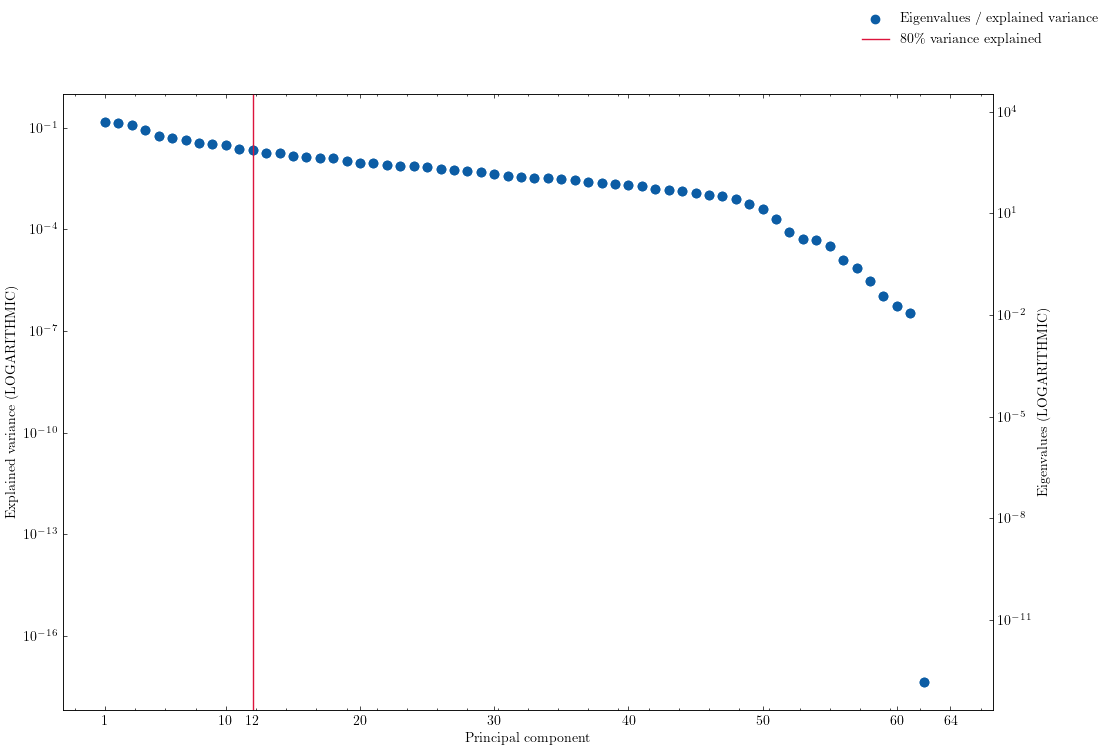
\includegraphics[width=0.8\textwidth]{figures/exp_var_eigenspectrum.png}
  \caption{\small \textit{Explained variance and Eigenspectrum}}
  \label{fig:exp_var}
\end{figure}


\subsubsection{Eigendigits}

In below \cref{fig:eigendigits} I plot the 5 most significant principal
components, or Eigendigits, as computed by running \texttt{my\_pca(X)} in the
code snippet shown earlier.

\begin{figure}[H]
  \centering
  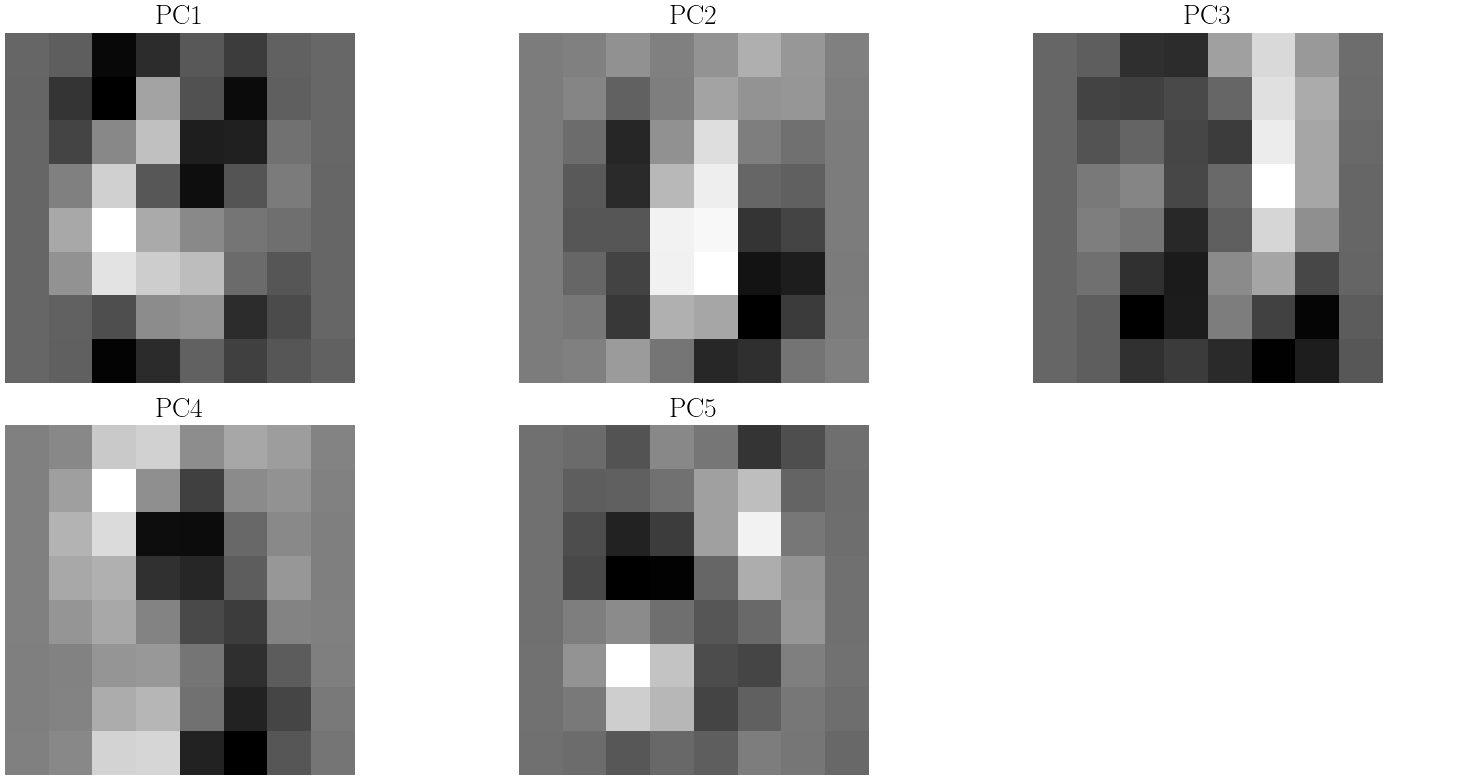
\includegraphics[width=0.8\textwidth]{figures/eigendigits.png}
  \caption{\small \textit{Five most significant eigendigits (ie. principal
  components)}}
  \label{fig:eigendigits}
\end{figure}

\sectend
